% This file was created with tikzplotlib v0.10.1.
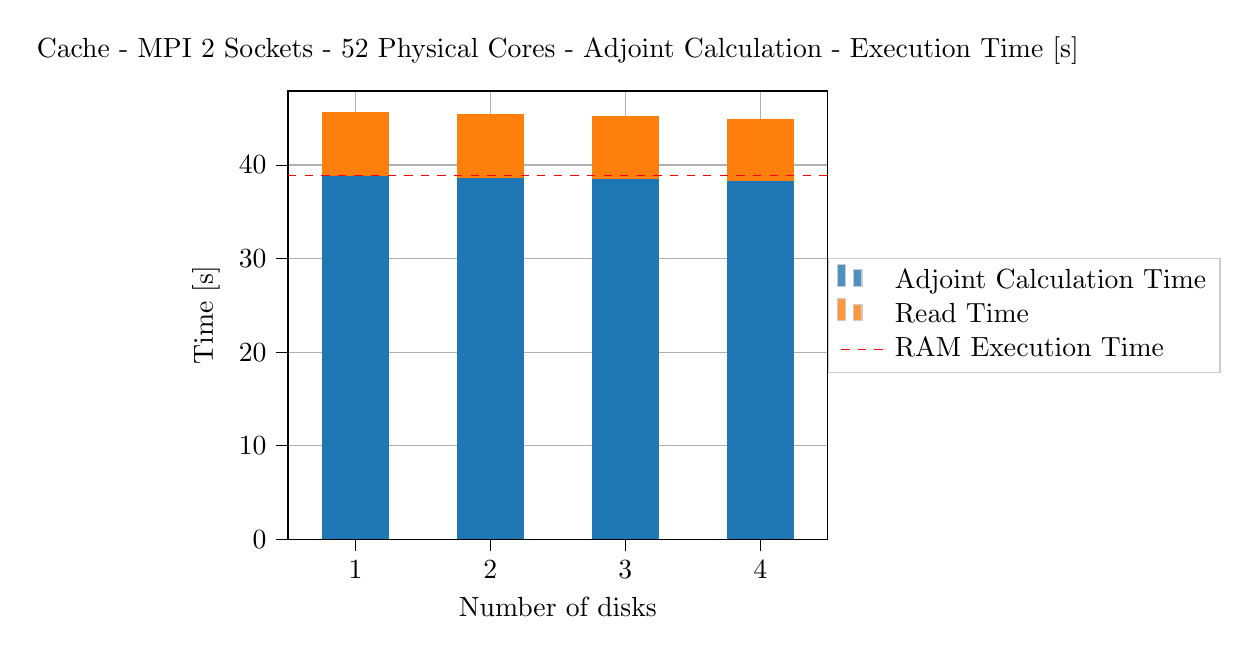
\begin{tikzpicture}

\definecolor{darkgray176}{RGB}{176,176,176}
\definecolor{darkorange25512714}{RGB}{255,127,14}
\definecolor{lightgray204}{RGB}{204,204,204}
\definecolor{steelblue31119180}{RGB}{31,119,180}

\begin{axis}[
legend cell align={left},
legend style={
  fill opacity=0.8,
  draw opacity=1,
  text opacity=1,
  at={(1,0.5)},
  anchor=west,
  draw=lightgray204
},
tick align=outside,
tick pos=left,
title={Cache - MPI 2 Sockets - 52 Physical Cores - Adjoint Calculation - Execution Time [s]},
x grid style={darkgray176},
xlabel={Number of disks},
xmajorgrids,
xmin=-0.5, xmax=3.5,
xtick style={color=black},
xtick={0,1,2,3},
xticklabels={1,2,3,4},
y grid style={darkgray176},
ylabel={Time [s]},
ymajorgrids,
ymin=0, ymax=47.9115,
ytick style={color=black}
]
\draw[draw=none,fill=steelblue31119180] (axis cs:-0.25,0) rectangle (axis cs:0.25,38.84);
\addlegendimage{ybar,ybar legend,draw=none,fill=steelblue31119180}
\addlegendentry{Adjoint Calculation Time}

\draw[draw=none,fill=steelblue31119180] (axis cs:0.75,0) rectangle (axis cs:1.25,38.66);
\draw[draw=none,fill=steelblue31119180] (axis cs:1.75,0) rectangle (axis cs:2.25,38.48);
\draw[draw=none,fill=steelblue31119180] (axis cs:2.75,0) rectangle (axis cs:3.25,38.24);
\draw[draw=none,fill=darkorange25512714] (axis cs:-0.25,38.84) rectangle (axis cs:0.25,45.63);
\addlegendimage{ybar,ybar legend,draw=none,fill=darkorange25512714}
\addlegendentry{Read Time}

\draw[draw=none,fill=darkorange25512714] (axis cs:0.75,38.66) rectangle (axis cs:1.25,45.41);
\draw[draw=none,fill=darkorange25512714] (axis cs:1.75,38.48) rectangle (axis cs:2.25,45.19);
\draw[draw=none,fill=darkorange25512714] (axis cs:2.75,38.24) rectangle (axis cs:3.25,44.91);
\addplot [semithick, red, dashed]
table {%
-0.5 38.88
3.5 38.88
};
\addlegendentry{RAM Execution Time}
\end{axis}

\end{tikzpicture}
